\subsection{Model parametrization}
\label{sec:param}
\subsubsection{Sea surface wind stress}


Equation 9 in Y20~\cite{ZannaPreprint} is,

\begin{equation}
 \boldsymbol{\tau} = C_d(|U_{10}|)\cdot \rho_{\mathrm{air}} \cdot U_{10}{}^2  \;{}\mathbf{\hat{U}_{10}}
 \label{eq:tau}
 \end{equation}

where $C_d$ is the drag coefficient, $\rho_{\mathrm{air}}$ is the density of the air,
$U_{10}$ is the wind speed 10m above the surface, and $\boldsymbol{\tau}$ is the sea surface stress.
 It is unclear whether how $C_d$ changes at high wind speeds
 \cite{powell2003reduced}, as initially roughness increases
 due to the waves, but this could decrease~\cite{powell2003reduced}
 or reach a limit~\cite{donelan2004limiting}.


\subsubsection{Sea surface wind induced heat transfer}

% 

    \begin{figure}
            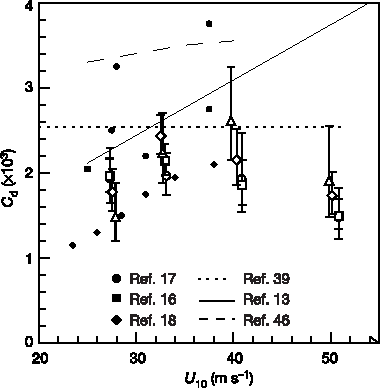
\includegraphics[width=1\linewidth]{images/example-images/cd.pdf}
                \caption{Fig. 3c from Powell 2003~\cite{powell2003reduced},
                 where they suggested that at high wind speeds $c_d$ decreases.}
    \end{figure}
\begin{figure}[htb!]
    \centering
    \includegraphics[width=1\linewidth]{../surge/plots/cd_finder.pdf}
    \caption{ Extracting $C_d$ from data.
    $ r_p = 0.9774 \pm 0.001,\;\; p<10^{-300}$\\
    $ m = 0.0383 \pm 0.0001 $ kg$^{0.5}$ m$^{-1.5}$\\
    $\implies  c_d = 0.001467 \pm 0.000008$ kg m$^{-3}$
    % error estimated from differences in output between test/training year,
    % measured regression error in either year much smaller than this.
    % The error is propogated using the \texttt{python3.uncertanties} package}
    There might be a theoretical limit~\cite{donelan2004limiting}.
    }
    %\label{fig:}
\end{figure}


Equation 4 in \cite{zou2017observation},

\begin{equation}
Q_{H}=
\rho_{\mathrm{air}} \cdot c_{p} \cdot C_{H}(|U_{10}|) \cdot
U_{10} \cdot \left(T_{\mathrm{air}}
-T_{\mathrm{ocean}}\right),
\end{equation}

where $Q_{H}$ is the heat transferred downwards, $c_p$ is the heat capacity of the air,
$C_{H}$ is the heat transfer coefficient,
$T_{\mathrm{air}}$ is the temperature of the atmosphere, and
$T_{\mathrm{ocean}}$ is the temperature of the ocean.
